\documentclass{beamer}
 
\usepackage[frenchb]{babel}
\usepackage[T1]{fontenc}
\usepackage[utf8]{inputenc}
\usepackage{upgreek}
\usepackage{amsmath}
\usepackage{amssymb}
\usepackage{pdfpages}
\usepackage[]{algorithm2e}
\usepackage[abs]{overpic}
\usepackage{mdwlist}
\usepackage{tikz}
\usepackage{hhline}
\usepackage{tikz}
\usepackage{subcaption}
\usepackage{tikz-qtree}
\usepackage{pbox}
\usepackage{forest}
\usepackage{slashbox}
\usepackage{hhline}
\usepackage{colortbl}
\usepackage{array}

\usetikzlibrary{trees}
\usetikzlibrary{babel}
\usetikzlibrary{arrows,automata,positioning}

\usepackage[style=alphabetic,backend=bibtex,autocite=footnote]{biblatex}

% \bibliographystyle{alpha}
\bibliography{biblio.bib}
\nocite{*}

\usetheme{Frankfurt}
  
\title{La phylogénie des images dans les réseaux sociaux}
\author{Noé LE PHILIPPE}
\institute{Équipe ICAR - William Puech}
\date{\today}
% \logo{\includegraphics[height=10mm]{images/logo.png}}

\addtobeamertemplate{navigation symbols}{}{%
    \usebeamerfont{footline}%
    \usebeamercolor[fg]{footline}%
    \hspace{1em}%
    \insertframenumber/\inserttotalframenumber
}

\AtBeginSection[]
{
  \begin{frame}
  \frametitle{Sommaire}
  \tableofcontents[currentsection, hideothersubsections]
  \end{frame} 
}

\makeatletter
\renewcommand\@makefnmark{\hbox{\@textsuperscript{\normalfont[\@thefnmark]}}}
\renewcommand\@makefntext[1]{{\normalfont[\@thefnmark]}\enspace #1}
\makeatother

\DeclareCiteCommand{\footfullcitetext}[\mkbibfootnotetext]
{\usebibmacro{prenote}}
{\usedriver
  {\DeclareNameAlias{sortname}{default}}
  {\thefield{entrytype}}}
{\multicitedelim}
{\usebibmacro{postnote}}

\newcolumntype{L}[1]{>{\raggedright\let\newline\\\arraybackslash\hspace{0pt}}m{#1}}
\newcolumntype{C}[1]{>{\centering\let\newline\\\arraybackslash\hspace{0pt}}m{#1}}
\newcolumntype{R}[1]{>{\raggedleft\let\newline\\\arraybackslash\hspace{0pt}}m{#1}}

\newenvironment<>{varblock}[2][.9\textwidth]{%
  \setlength{\textwidth}{#1}
  \begin{actionenv}#3%
    \def\insertblocktitle{#2}%
    \par%
    \usebeamertemplate{block begin}}
  {\par%
    \usebeamertemplate{block end}%
  \end{actionenv}}

\begin{document}

\begin{frame}
  \titlepage
\end{frame}

\section{Introduction}
\begin{frame}
  \frametitle{Le sujet de stage}

  \begin{block}{Le sujet}
    La phylogénie des images dans les réseaux sociaux
  \end{block}
  \pause
  \begin{block}{Définition}
    {\large ``La phylogenèse ou phylogénie est l'étude des relations de parenté entre êtres vivants.''}
    \hspace*\fill{\small--- Wikipedia}
  \end{block}

\end{frame}

\begin{frame}
  \frametitle{Les applications}
  \begin{block}{}
    Réduire le nombre de versions de la même image pour optimiser l'espace de stockage
  \end{block}
  \pause
  \begin{block}{}
    Suivre l'évolution et la diffusion d'images sur les réseaux sociaux
  \end{block}
  \pause
  \begin{block}{}
    Détecter l'altération d'images
  \end{block}
\end{frame}

\begin{frame}
  \frametitle{Définitions}

  \begin{block}{Near-Duplicate Image (NDI)\footnotemark}
    Une image I\textsubscript{n} est le near-duplicate d'une image I\textsubscript{m} si :
    $$I_{n} = T(I_{m}), T \in \mathcal{T}$$
    où $\mathcal{T}$ est un ensemble de transformations autorisées
  \end{block}
  \footfullcitetext{joly2007content}
  Dans le cas général, 
  \begin{multline*}
    \mathcal{T} = \{resampling, cropping, affine\ warping,\\ color\ changing, lossy\ compression\}
  \end{multline*}
  mais dans le cadre du stage, $\mathcal{T} = \{lossy\ compression\}$
\end{frame}

\begin{frame}
  \frametitle{Définitions}
  \begin{block}{Image Phylogeny Tree (IPT)}
    C'est l'arbre retraçant la parenté des images
  \end{block}

  \begin{center}
      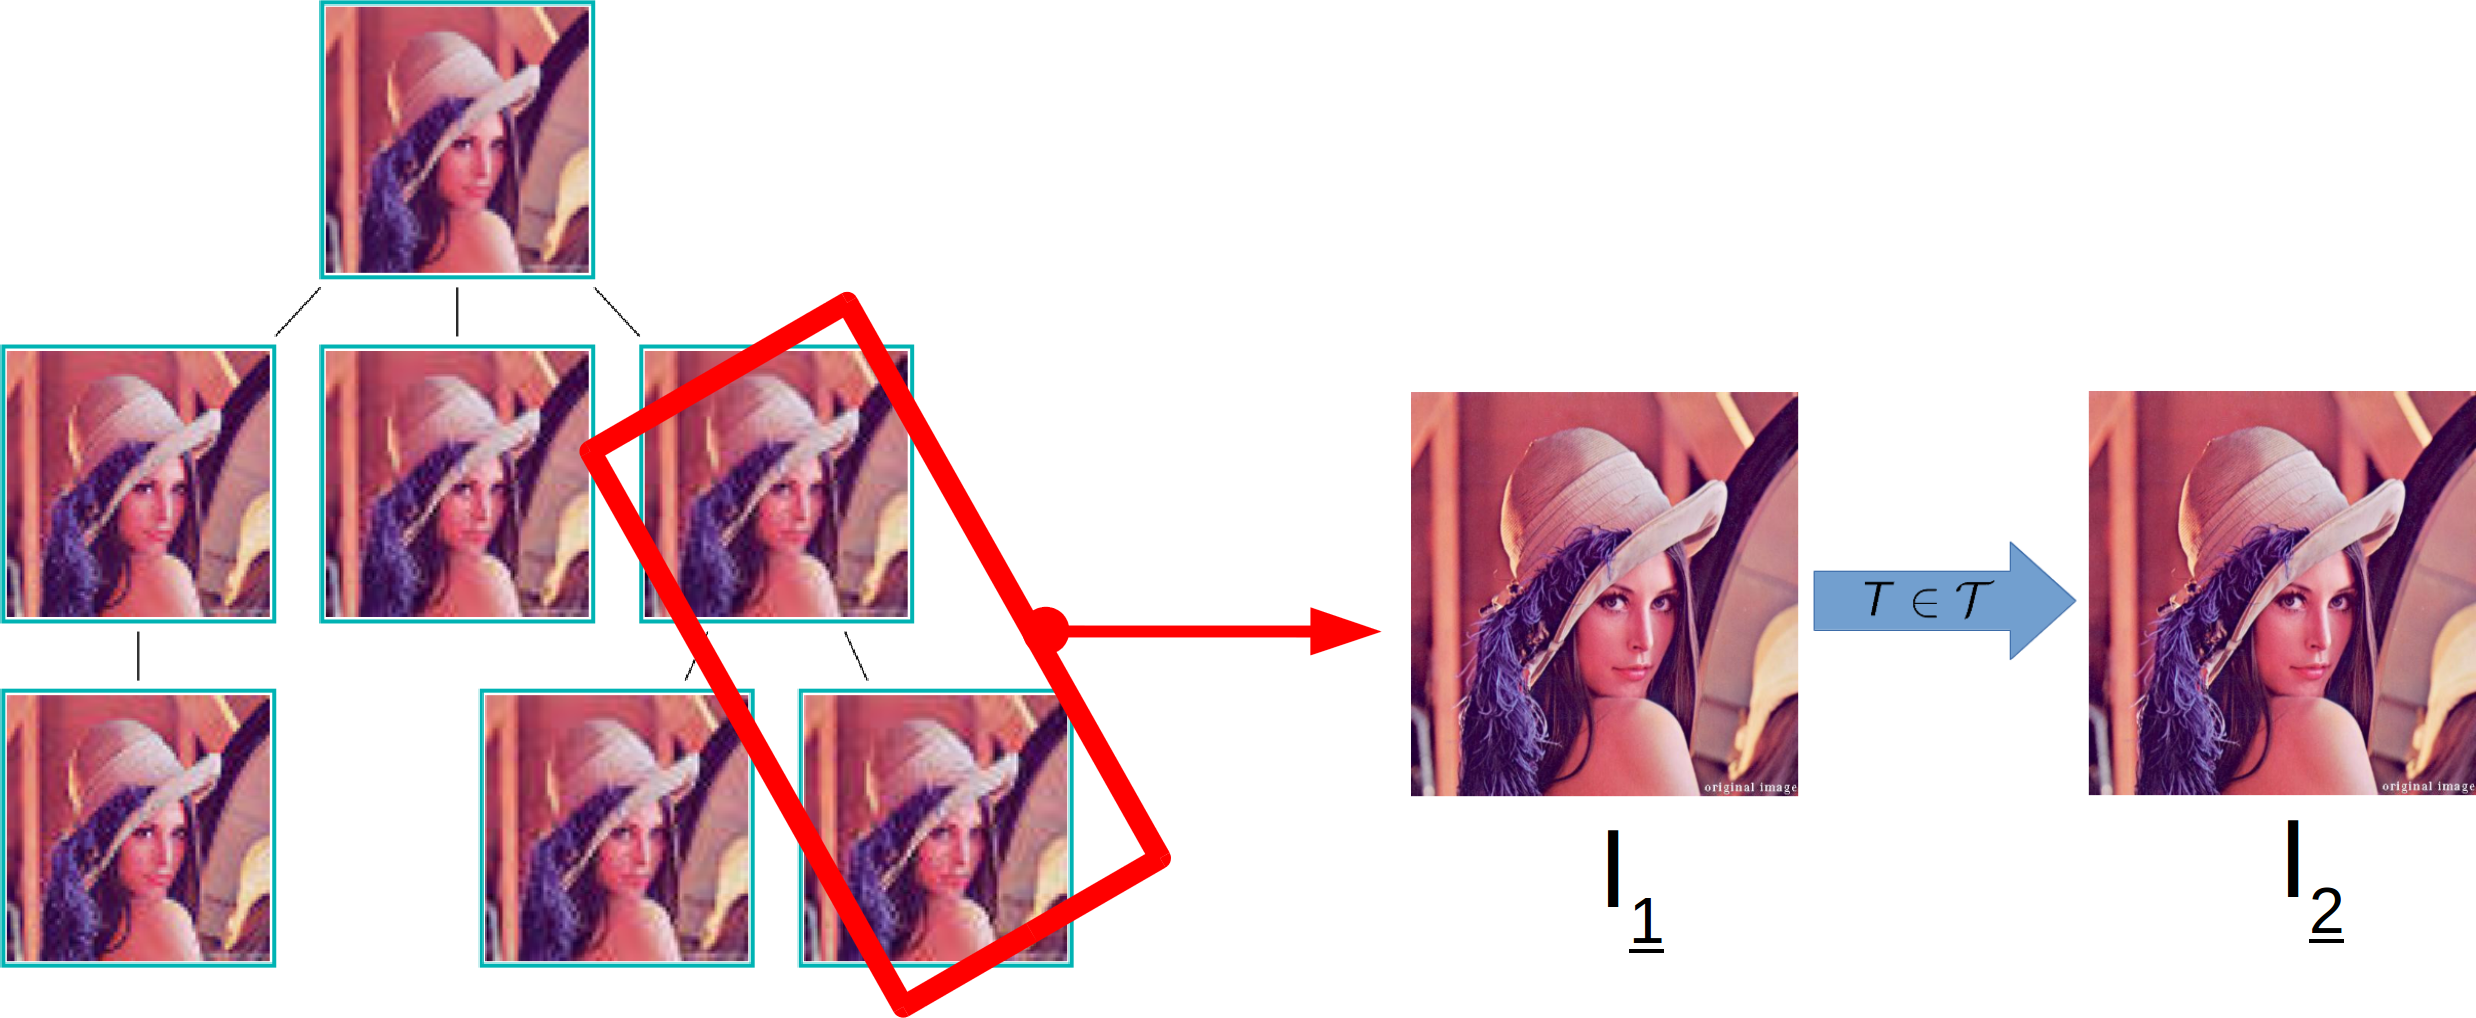
\includegraphics[width=1\textheight]{tree_extract.png}
  \end{center}

\end{frame}

\begin{frame}
  \frametitle{Image phylogeny tree}
  \begin{center}
    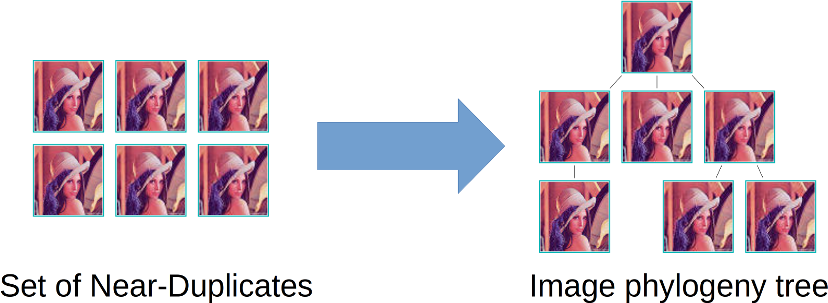
\includegraphics[width=0.8\textwidth]{set_to_tree.png}
  \end{center}
  Deux parties importantes lors de la reconstruction de l'arbre phylogénétique : 
  \pause
  \begin{columns}
    \begin{column}{0.5\textwidth}
      \begin{block}{}
        \begin{itemize}
        \item Correctement identifier la racine
        \end{itemize}
      \end{block}
      \pause
    \end{column}
    \begin{column}{0.5\textwidth}
      \begin{block}{}
        \begin{itemize}
        \item Estimer au mieux l'arborescence
        \end{itemize}
      \end{block}
    \end{column}
  \end{columns}
\end{frame}

\begin{frame}
  \frametitle{Notre cas d'étude}
        \scalebox{0.6}{%
      \begin{tikzpicture}[auto,node distance=2.8cm]

        \tikzstyle{every state}=[shape=rectangle,minimum width=1.3in,text width=1.3in, align=center,fill=blue!30]

        \node[draw=none,fill=none] (A) {image originale};
        \node[state] (B) [right=0.7cm of A] {première compression JPEG avec $Q_{1}$};
        \node[draw=none,fill=none,minimum width=1.1in,text width=1.1in] (C) [right=0.7cm of B] {première image compressée};
        \node[state] (D) [above right=1.7cm and 0.9cm of C] {$n^{ieme}$ compression JPEG avec $Q_{n+1} = Q_{n}$};
        \node[shape=rectangle,minimum width=1.3in,text width=1.3in, align=center,fill=green!90] (E) [right=0.9cm of C] {$n^{ieme}$ compression JPEG avec $Q_{n+1} < Q_{n}$};
        \node[state] (F) [below right=1.7cm and 0.9cm of C] {$n^{ieme}$ compression JPEG avec $Q_{n+1}\ \{<,>,=\}\ Q_{n}$};
        \node[draw=none,fill=none,minimum width=0.79in,text width=0.79in] (G) [right=0.7cm of D] {$n^{ieme}$ image compressée};
        \node[draw=none,fill=none,minimum width=0.79in,text width=0.79in] (H) [right=0.7cm of E] {$n^{ieme}$ image compressée};
        \node[draw=none,fill=none,minimum width=0.79in,text width=0.79in] (I) [right=0.7cm of F] {$n^{ieme}$ image compressée};

        \node[draw=none,fill=none] (D1) [below=0.7cm of D] {};
        \node[draw=none,fill=none] (D2) [below=0.94cm of G] {};

        \node[draw=none,fill=none] (E1) [below=0.7cm of E] {};
        \node[draw=none,fill=none] (E2) [below=0.94cm of H] {};

        \node[draw=none,fill=none] (F1) [below=0.7cm of F] {};
        \node[draw=none,fill=none] (F2) [below=0.94cm of I] {};

        
        \path [->] (A) edge node[left] {} (B);
        \path [->] (B) edge node[left] {} (C);      
        \path [->] (C.east) edge node[left] {} (D.west);
        \path [->] (C.east) edge node[left] {} (E.west);
        \path [->] (C.east) edge node[left] {} (F.west);
        \path [->] (D) edge node[left] {} (G);
        \path [->] (E) edge node[left] {} (H);
        \path [->] (F) edge node[left] {} (I);

        \path [->] (D1.center) edge node[left] {} (D);
        \path [-] (D2.center) edge node[left] {} (D1.center);
        \path [-] (G.south) edge node[left] {} (D2.center);

        \path [->] (E1.center) edge node[left] {} (E);
        \path [-] (E2.center) edge node[left] {} (E1.center);
        \path [-] (H.south) edge node[left] {} (E2.center);

        \path [->] (F1.center) edge node[left] {} (F);
        \path [-] (F2.center) edge node[left] {} (F1.center);
        \path [-] (I.south) edge node[left] {} (F2.center);
      \end{tikzpicture}}
\end{frame}

\section{État de l'art}

\begin{frame}
  \frametitle{Estimation de l'arbre de phylogenie}

  \only<1,3,5> {
    \begin{block}{Visual Migration Map\footnotemark}
      \begin{itemize}
      \item Les transformations sont directionnelles
      \item Relation parent-enfant si tous les détecteurs s'accordent sur la direction
      \item Simplification du graphe par sélection des plus longs chemins
      \end{itemize}
    \end{block}
    \footfullcitetext{kennedy2008internet}
  }
  \only<2> {
    \begin{center}
      \includegraphics<2>[scale=0.3]{vmm}
    \end{center}
  }
  \only<4> {
    \begin{center}
      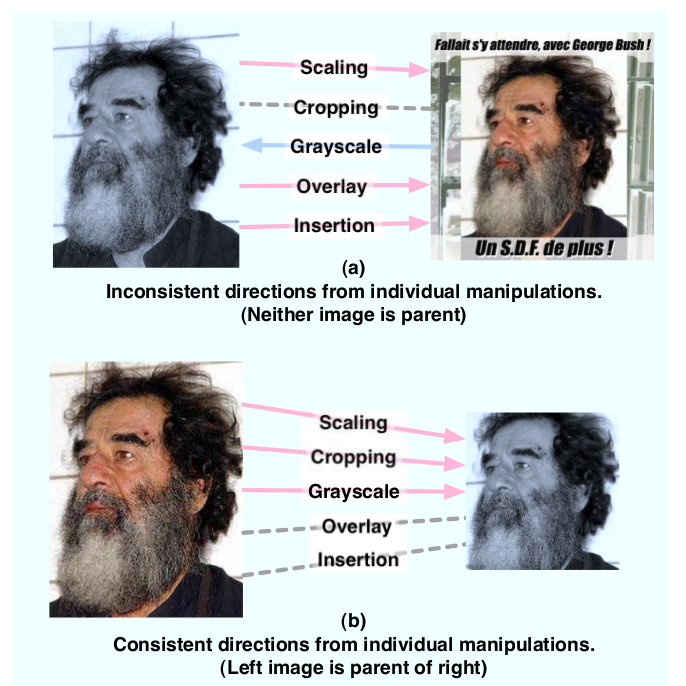
\includegraphics[scale=0.3]{vmm_directionnel}
    \end{center}
  }
  \only<6> {
    \begin{center}
      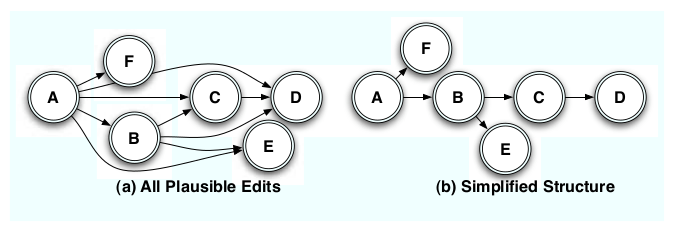
\includegraphics[scale=0.45]{vmm_tree}
    \end{center}
  }
\end{frame}

\begin{frame}
  \frametitle{Estimation de l'arbre de phylogénie}
  \begin{block}{Image phylogeny tree \footnotemark[3] \footnotemark[4]}
    \begin{itemize}
      \item Calcul d'une \textit{dissimilarity matrix}
      \item Calcul d'un arbre couvrant de poids min (Kruskal ou autre)
    \end{itemize}
  \end{block}
  \stepcounter{footnote}
  \stepcounter{footnote}
  \footfullcitetext{dias2010first}
  \stepcounter{footnote}
  \footfullcitetext{dias2012image}
\end{frame}

% \section{Analyse des recompressions}
\begin{frame}
  \frametitle{Convergence des blocs lors de compressions successives \footnotemark[5]}
  \begin{block}{But}
    Compter le nombre de compressions
  \end{block}
  \begin{block}{3 types de blocs}
    \begin{itemize}
      \item Les blocs plats
      \item Les blocs stables
      \item Les blocs cycliques
    \end{itemize}
  \end{block}  
  \begin{block}{Comment ?}
    plus petit commun multiple de la longueur des cycles
  \end{block}
  \stepcounter{footnote}
  \footfullcitetext{CarneinSB2016TelltaleWatermarks}
\end{frame}

\begin{frame}
  \frametitle{Convergence des blocs lors de compressions successives}
  \centering
  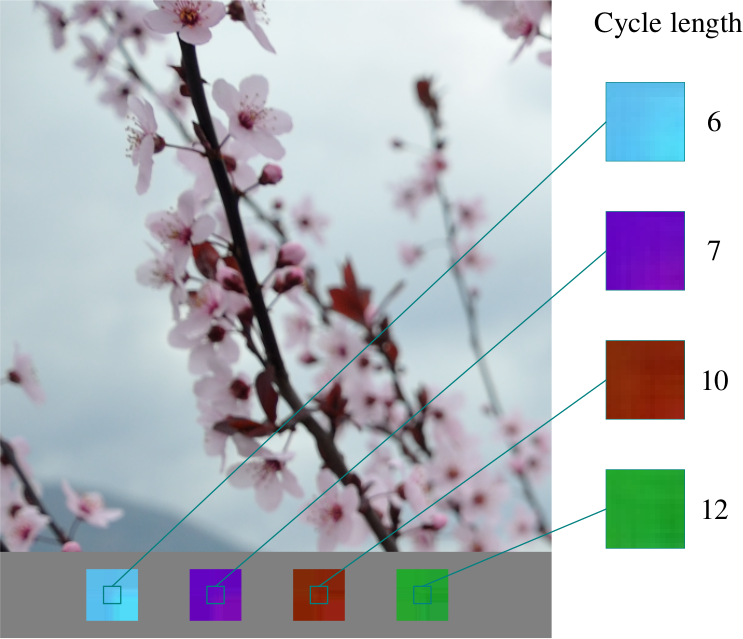
\includegraphics[scale=0.3]{insertion_blocs}
 
\end{frame}

% \begin{frame}
%   \frametitle{Convergence des blocs lors de compressions successives}
   
%     \only<1,2>{
%       \begin{block}{Utilisation des blocs}
%         \begin{itemize}
%         \item Les blocs de l'image
%         \item Insérer des blocs
%         \end{itemize}
%       \end{block}
%       \pause
%       \begin{block}{Les inconvénients}
%         \begin{itemize}
%         \item Nécessite du padding
%         \item Limité à la même table de quantification
%         \item Résultats moyens pour $Q_f$ < 100
%         \end{itemize}
%       \end{block}  
%     }

%   % \footfullcite{CarneinSB2016TelltaleWatermarks}
% \end{frame}

\begin{frame}
  \frametitle{Estimation de la matrice de quantification primaire \footnotemark[6]}
  \begin{block}{Principe de leur méthode}
    Comparer l'histogramme de l'image originale et l'histogramme des images compressées avec des tables de quantification modèles puis compressées avec $Q_{f_2}$ et enfin garder la table pour laquelle la différence entre histogramme est la plus faible
  \end{block}
  \stepcounter{footnote}
  \footfullcitetext{lukavs2003estimation}
\end{frame}

\begin{frame}
\centering
\begin{columns}[T] % align columns
\begin{column}{.48\textwidth}
  \begin{block}{Analyse des valeurs manquantes}
    Artefacts distincts pour $Q_{f_1} > Q_{f_2}$ et $Q_{f_1} < Q_{f_2}$
  \end{block}

  \begin{block}{Limites}
    \begin{itemize}
    \item $Q_{f_1} = Q_{f_2}$
    \item $Q_{f_1}$ est facteur de $Q_{f_2}$
    \end{itemize}
  \end{block}

  % \hfill
  \hspace*{-3.4mm}
  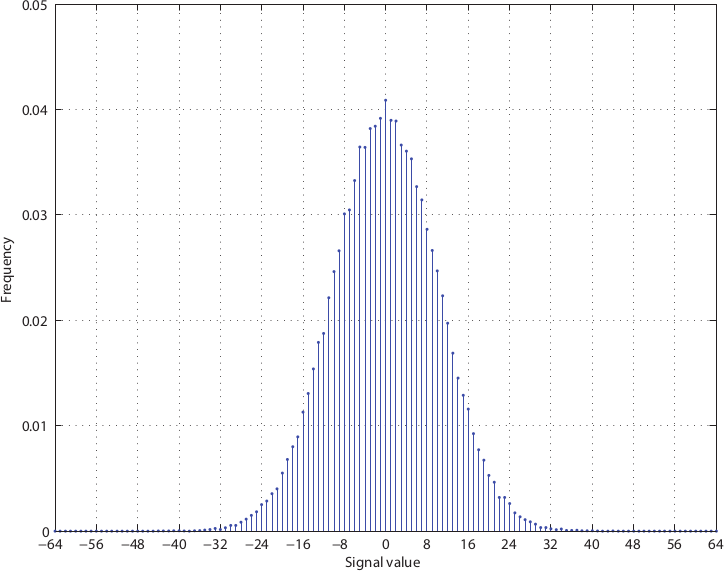
\includegraphics[height=0.475\textheight]{h1}
\end{column}%
\hfill%
\begin{column}{.48\textwidth}
  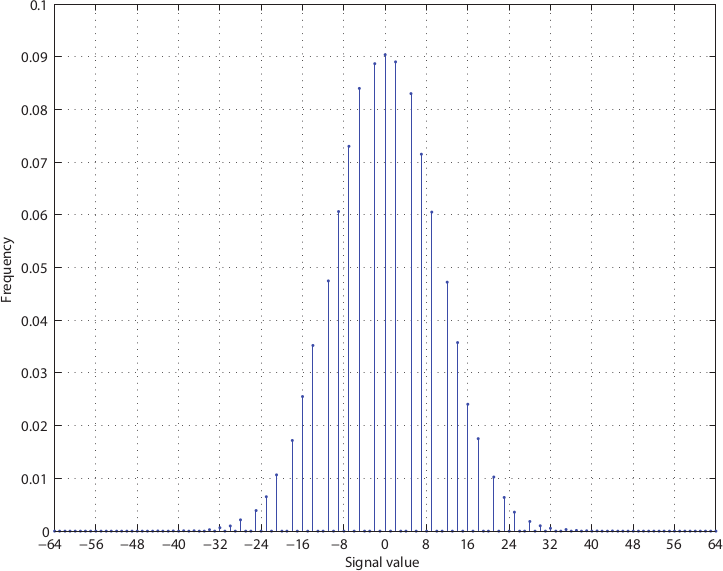
\includegraphics[height=0.475\textheight]{h2}
  \hfill
  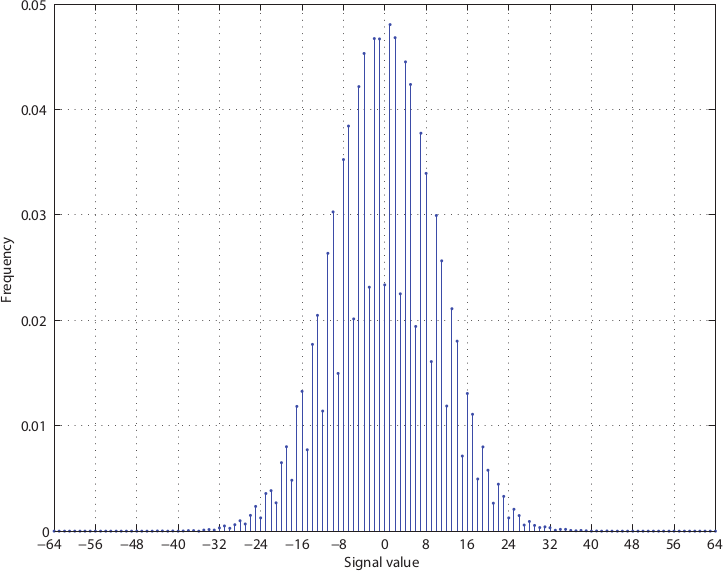
\includegraphics[height=0.475\textheight]{h3}
\end{column}%
\end{columns}
\end{frame}


% \begin{frame}
%   \frametitle{Estimation de la matrice de compression primaire}
%   \begin{block}{Analyse des valeurs manquantes de l'histogramme}
%     Artefacts distincts pour $Q^{1} > Q^{2}$ et $Q^{1} < Q^{2}$
%   \end{block}
%   \pause
%   \begin{block}{Limites}
%     \begin{itemize}
%     \item $Q^{1} \neq Q^{2}$
%     \item $Q^{1}$ n'est pas facteur de $Q^{2}$
%     \end{itemize}
%   \end{block}
% \end{frame}


\section{Notre approche}

\begin{frame}
  \begin{block}{But}
    Réduction d'un problème de reconstruction d'un arbre de phylogénie à un problème de \textbf{négation de parenté}
  \end{block}
  \begin{block}{Solution}
    Décision binaire entre deux images : ``Cette image est-elle le parent de cette autre image ?''
  \end{block}
\end{frame}

\begin{frame}
  \frametitle{Notre approche}
  \begin{block}{Marqueur}
    Caractéristique de l'image qui indique qu'une certaine opération a été effectuée et qui va se transmettre aux enfants
  \end{block}
  \pause
  \begin{block}{Fonction de négation}
  $f(I_{m},I_{n})$ est une fonction qui pour tout couple d'images $(I_{m}, I_{n})$ détecte à chaque fois qu'il est présent un marqueur visible dans une image et pas dans l'autre, et donc prouve qu'il n'y a pas de relation de parenté entre $I_{m}$ et $I_{n}$.
    % $f(I_{m}, I_{n})$ est une fonction qui pour tout couple d’images (I\textsubscript{m}, I\textsubscript{n}) détecte à chaque fois qu’il est présent un marqueur indiquant qu’il n’y a pas de relation de parenté entre I\textsubscript{m} et I\textsubscript{n}.
  \end{block}
  \pause
  \begin{block}{Théorème}
  Pour tout couple d'images ($I_{m}$, $I_{n}$) d'un ensemble de near-duplicates, s'il n'existe pas de marqueur prouvant que $I_{m}$ n'est pas le parent de $I_{n}$, alors il y a une relation parent-enfant entre $I_{m}$ et $I_{n}$, $I_{m}$ $\to$ $I_{n}$.
     % Pour tout couple d'images ($I_{m}$, $I_{n}$) d'un ensemble de near-duplicates, s'il n'existe pas de marqueur prouvant que $I_{m}$ n'est pas le parent de $I_{n}$, alors il y a une relation parent-enfant entre $I_{m}$ et $I_{n}$, $I_{m}$ $\to$ $I_{n}$.
  \end{block}
  % \begin{itemize}
  % \item Tentative de preuve qu'une image n'est pas le parent d'une autre
  % \item Si c'est impossible, l'image doit alors être le parent
  % \item Extraction d'une \textit{matrice de parenté}
  % \item Calcul de l'arbre
  % \end{itemize}
  % \end{block}
\end{frame}

\begin{frame}
  \frametitle{Schéma de notre approche}
  \begin{figure}[H]
    \centering
    % \begin{tikzpicture}[auto, distance=2in,sibling distance=.25in]
    \scalebox{0.55}{
      \begin{tikzpicture}[auto,node distance=2.8cm]

        \tikzstyle{every state}=[shape=rectangle,minimum width=1.3in,text width=1.3in, align=center,fill=blue!30]
        % \tikzstyle{every data}=[shape=circle,minimum width=1.3in,text width=1.3in, align=center,fill=blue!30]

        \node[draw=none,fill=none,minimum width=1.1in,text width=1.1in, align=center] (A) {Ensemble de near-duplicates};
        \node[state] (B) [right=0.7cm of A] {DCT sur chaque image};

        \node[draw=none,fill=none,minimum width=1.1in,text width=1.1in, align=center, right=0.7cm of B] (C) {Coeffs DCT de chaque image};
        \node[state] (D) [right=0.7cm of C] {Extraction de la période de chaque coefficient DCT};

        \node[draw=none,fill=none,minimum width=1.1in,text width=1.1in, align=center, right=0.7cm of D] (E) {Tables de quantification estimées};
        \node[state] (F) [below=0.7cm of E] {Estimation du facteur de qualité};

        \node[draw=none,fill=none,minimum width=1.1in,text width=1.1in, align=center, left=0.7cm of F] (G) {$Q_f$ de chaque image};
        \node[draw=none,fill=none,minimum width=1.1in,text width=1.1in, align=center, below=0.3cm of G] (H) {Images};
        \node[state] (I) [left=0.7cm of G] {Estimation du parent};

        \node[draw=none,fill=none,minimum width=1.1in,text width=1.1in, align=center, left=0.7cm of I] (J) {Matrice de parenté};
        \node[state] (K) [left=0.7cm of J] {Construction de l'arbre};

        \node[draw=none,fill=none,minimum width=1.1in,text width=1.1in, align=center, below=1.2cm of K] (L) {Arbre non traité};
        \node[state] (M) [right=0.7cm of L] {Filtrage des doublons};
        
        \node[draw=none,fill=none,minimum width=1.1in,text width=1.1in, align=center, right=0.7 of M] (N) {Arbre de phylogénie};

        \path [->] (A) edge node[left] {} (B);
        \path [->] (B) edge node[left] {} (C);      
        \path [->] (C) edge node[left] {} (D);      
        \path [->] (D) edge node[] {} (E);      
        \path [->] (E) edge node[right] {} (F);      
        \path [->] (F) edge node[right] {} (G);      
        \path [->] (G) edge node[left] {} (I); 
        \path [->] (H) edge node[left] {} (I);
        \path [->] (I) edge node[left] {} (J);
        \path [->] (J) edge node[left] {} (K);
        \path [->] (K) edge node[left] {} (L);
        \path [->] (L) edge node[left] {} (M);
        \path [->] (M) edge node[left] {} (N);
      \end{tikzpicture}}
    % \caption{Schéma général de notre méthode.}
    \label{fig:method_schema}
  \end{figure}
\end{frame}

\begin{frame}
  \frametitle{Extraction de la période}
  \begin{block}{Qu'est ce que la période}
    Delta entre chaque pic de l'autocorrélation
  \end{block}
  \centering
  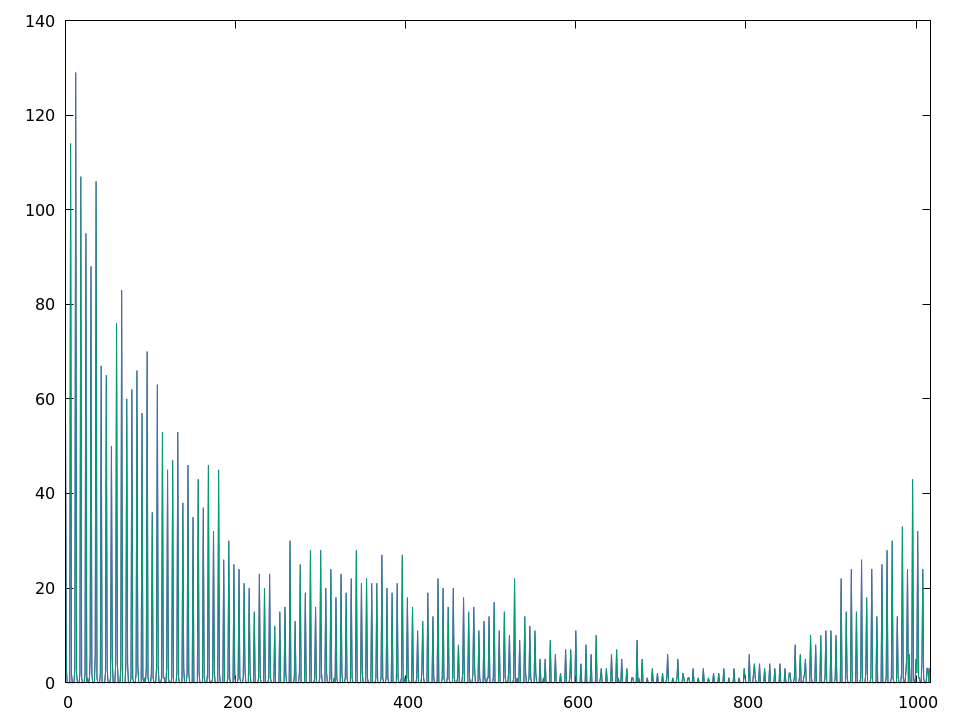
\includegraphics[width=0.5\linewidth]{signal.png}
  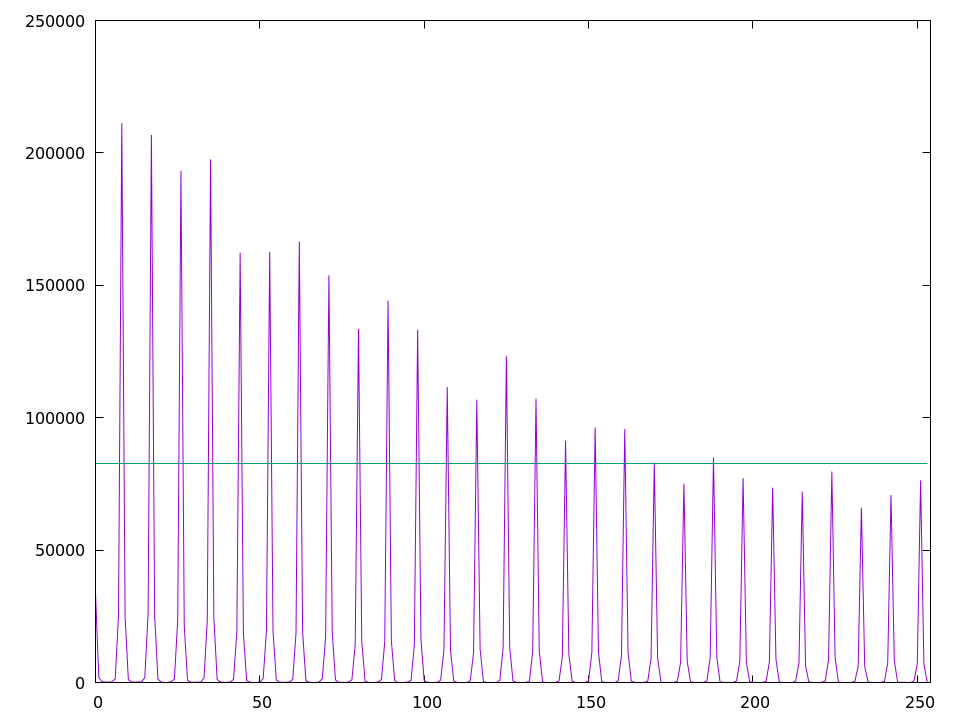
\includegraphics[width=0.5\linewidth]{autocorrelation.png}
\end{frame}

% \cellcolor{gray!25}

\begin{frame}
  \frametitle{Extraction de la période}
  \begin{figure}
    \centering
    \begin{tabular}{|c|c|c|c|c|c|c|c|}
      \hline
      9 & 6 & 5 & 9 & 13 & 22 & 22 & 30 \\ \hline    
      6 & 6 & 8 & 10 & 14 & 16 & 30 & \cellcolor{gray!25} \\ \hline
      8 & 7 & 9 & 13 & 20 & 31 & \cellcolor{gray!25} & \cellcolor{gray!25} \\ \hline
      8 & 9 & 12 & 19 & 28 & \cellcolor{gray!25} & \cellcolor{gray!25} & \cellcolor{gray!25} \\ \hline
      10 & 12 & -1 & -1 & \cellcolor{gray!25} & \cellcolor{gray!25} & \cellcolor{gray!25} & \cellcolor{gray!25} \\ \hline
      12 & 13 & 30 & \cellcolor{gray!25} & \cellcolor{gray!25} & \cellcolor{gray!25} & \cellcolor{gray!25} & \cellcolor{gray!25} \\ \hline
      28 & 31 & \cellcolor{gray!25} & \cellcolor{gray!25} & \cellcolor{gray!25} & \cellcolor{gray!25} & \cellcolor{gray!25} & \cellcolor{gray!25} \\ \hline
      \cellcolor{gray!25} & \cellcolor{gray!25} & \cellcolor{gray!25} & \cellcolor{gray!25} & \cellcolor{gray!25} & \cellcolor{gray!25} & \cellcolor{gray!25} & \cellcolor{gray!25} \\ \hline
    \end{tabular}
    \caption{Exemple de table de quantification retournée par l'estimation de la période, $\widehat{q}(u,v)$.}
    \label{periods1}
  \end{figure}
  \begin{block}{}
    Limitation au 35 premiers coefficients
  \end{block}
\end{frame}

\begin{frame}
  \frametitle{Extraction de la période}
  \centering
  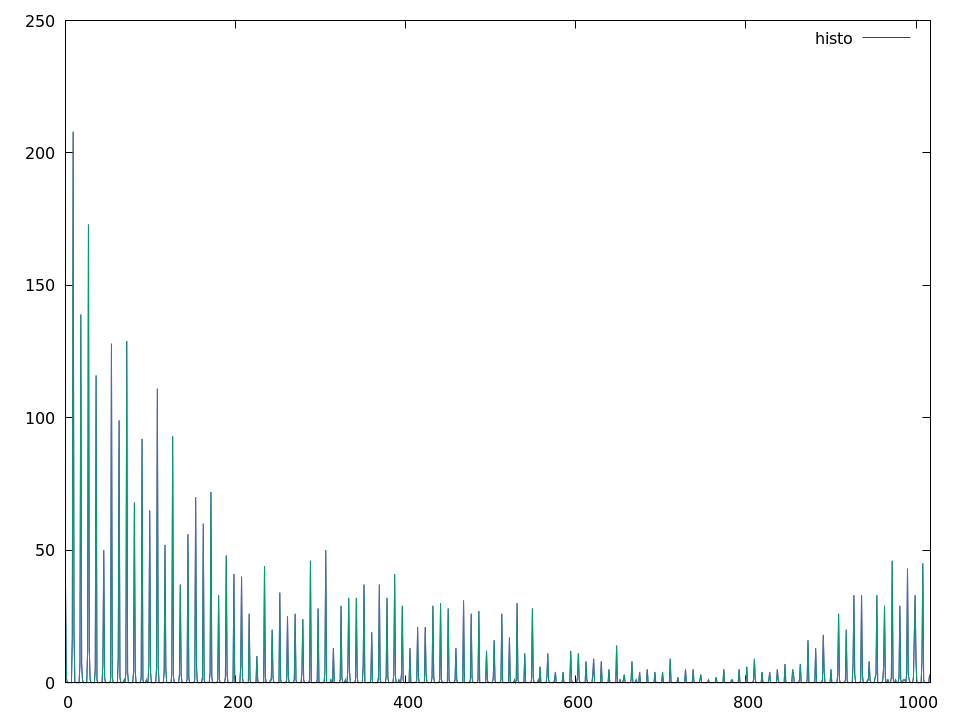
\includegraphics[width=0.45\linewidth]{histo0.png}
  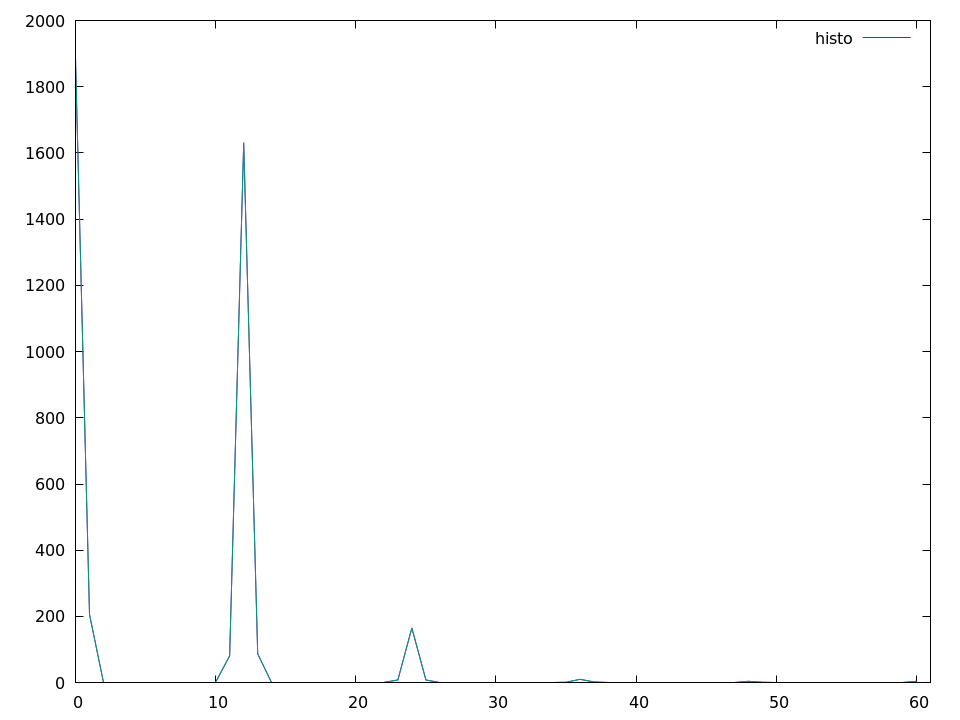
\includegraphics[width=0.45\linewidth]{histo18.png}


  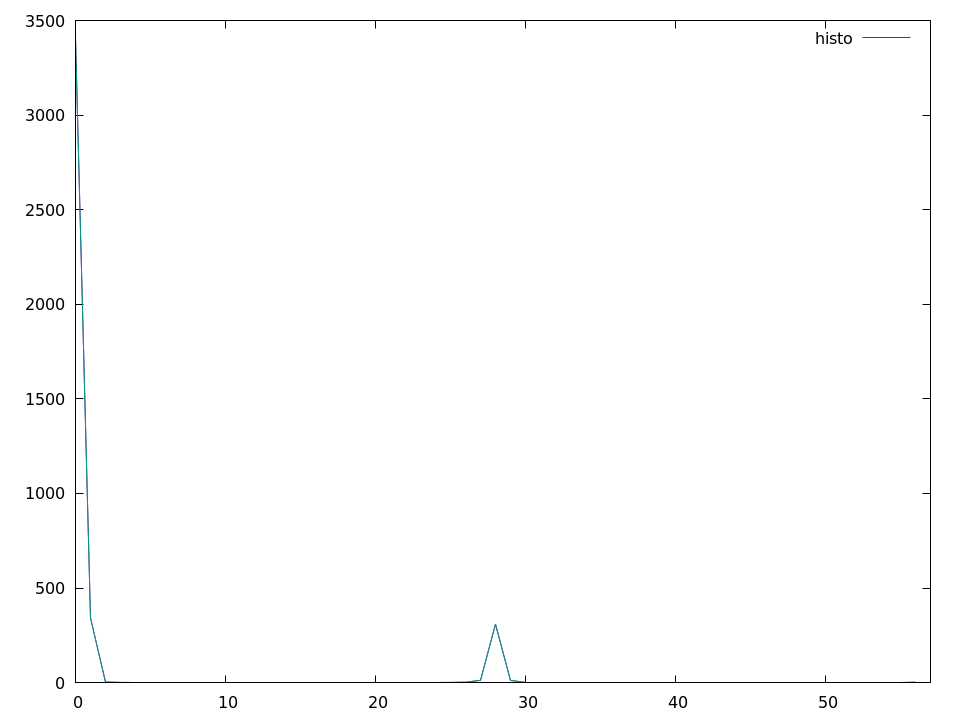
\includegraphics[width=0.45\linewidth]{histo31.png}
  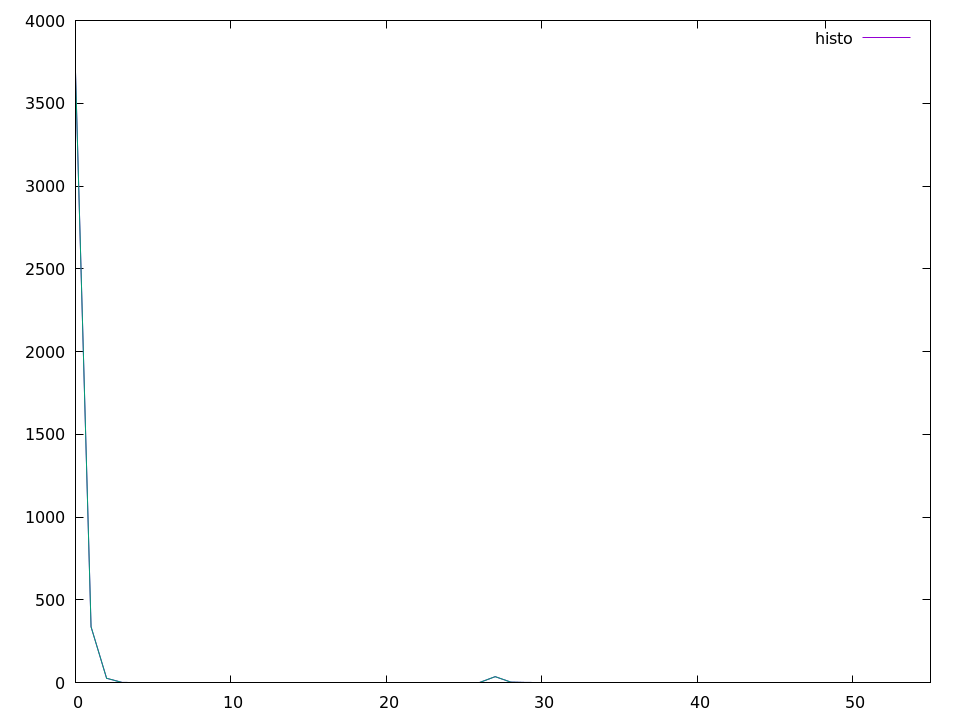
\includegraphics[width=0.45\linewidth]{histo40.png}
\end{frame}

\begin{frame}
  \frametitle{Estimation du facteur de qualité : estimation primaire}
  \begin{block}{Estimation primaire}
    Calcul de distance entre $\widehat{q}(u,v)$ et table(i) : $D_{euc}(P,Q) = \sqrt{\sum\limits_{i=1}^{d}|P_{i} - Q_{i}|^2}$
  \end{block}
  \begin{block}{Avantage}
    Donne directement $Q_f$
  \end{block}
  \begin{block}{Inconvénients}
    \begin{itemize}
    \item Lent
    \item Imprécise
    \end{itemize}
  \end{block}
\end{frame}

\begin{frame}
  \frametitle{Estimation du facteur de qualité : estimation primaire}
  \centering
  \begin{figure}
    \begin{subfigure}{0.7\linewidth}
    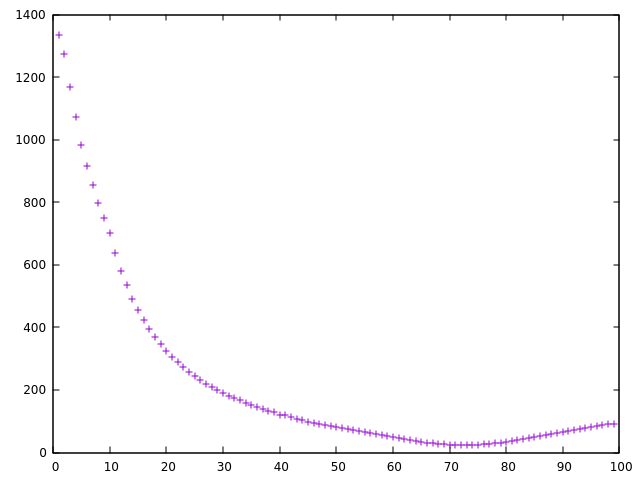
\includegraphics[width=0.95\linewidth]{distances.png}
    \end{subfigure}%
    \begin{subfigure}{0.3\linewidth}
    \scalebox{0.5}{
      \centering
      \begin{tabular}{| C{0.58cm} | C{0.58cm} | C{0.58cm} | C{0.58cm} | C{0.58cm} | C{0.58cm} | C{0.58cm} | C{0.58cm} |}
        \hline
        32&24&28&28&36&48&98&144\\ \hline
        22&24&26&34&44&70&128&184\\ \hline
        20&28&32&44&74&110&156&190\\ \hline
        32&38&48&58&112&128&174&196\\ \hline
        48&52&80&102&136&162&206&224\\ \hline
        80&116&114&174&218&208&242&200\\ \hline
        102&120&138&160&206&226&240&206\\ \hline
        122&110&112&124&154&184&202&198\\ \hline
      \end{tabular}}
    \vspace{5mm}    

    \scalebox{0.5}{
      \begin{tabular}{| C{0.58cm} | C{0.58cm} | C{0.58cm} | C{0.58cm} | C{0.58cm} | C{0.58cm} | C{0.58cm} | C{0.58cm} |}
        \hline
        16&12&14&14&18&24&49&72\\ \hline
        11&12&13&17&22&35&64&92\\ \hline
        10&14&16&22&37&55&78&95\\ \hline
        16&19&24&29&56&64&87&98\\ \hline
        24&26&40&51&68&81&103&112\\ \hline
        40&58&57&87&109&104&121&100\\ \hline
        51&60&69&80&103&113&120&103\\ \hline
        61&55&56&62&77&92&101&99\\ \hline
      \end{tabular}}
    \vspace{5mm}    

    \scalebox{0.5}{ 
      \begin{tabular}{| C{0.58cm} | C{0.58cm} | C{0.58cm} | C{0.58cm} | C{0.58cm} | C{0.58cm} | C{0.58cm} | C{0.58cm} |}
        \hline
        8&6&7&7&9&12&25&36\\ \hline
        6&6&7&9&11&18&32&46\\ \hline
        5&7&8&11&19&28&39&48\\ \hline
        8&10&12&15&28&32&44&49\\ \hline
        12&13&20&26&34&41&52&56\\ \hline
        20&29&29&44&55&52&61&50\\ \hline
        26&30&35&40&52&57&60&52\\ \hline
        31&28&28&31&39&46&51&50\\ \hline
      \end{tabular}}
    \end{subfigure}
  \end{figure}

\end{frame}

\begin{frame}
  \frametitle{Estimation du facteur de qualité : estimation secondaire}
  \begin{block}{Estimation secondaire}
    Utilisation des formules 
  \end{block}
  \begin{block}{Avantages}
    \begin{itemize}
      \item Rapide
      \item Précise
    \end{itemize}
  \end{block}
  \begin{block}{Inconvénients}
    $Q_f$ est nécessaire pour calculer $Q_f$
  \end{block}

\begin{equation}
 Si\ \ \  Q_f < 50\ \ \ \  Q_s = 5000 / Q_f  \ \ sinon \ \ Q_s = 200 - (Q_f \times 2)
\label{eqn:jpeg_1}
\end{equation}

\begin{equation}
\begin{split}
  q(u,v) = \frac{(base(u,v) \times Q_s) - 50}{100}\ \ \  avec\ \ \ 1 \leq q(u,v) \leq 255
\end{split}
  \label{eqn:jpeg_2}
\end{equation}
\end{frame}

\begin{frame}
  \frametitle{Estimation des ancêtres}
  \begin{block}{}
    La compression est déterministe
  \end{block}
  \begin{block}{}
    La compression n'est pas transitive
  \end{block}
  \begin{block}{}
    Le parent est à une compression de distance de ses enfants
  \end{block}
  \begin{block}{}
    Suppression des images ne pouvant pas être un ancêtre
  \end{block}
  \begin{block}{}
    Décision binaire
  \end{block}
\end{frame}

\begin{frame}
  \frametitle{Reconstruction de l'arbre}
  \begin{block}{}
    Matrice binaire de taille $n \times n$
  \end{block}
  \begin{block}{}
    Construction de l'arbre à partir de la matrice
  \end{block}
\begin{figure}
  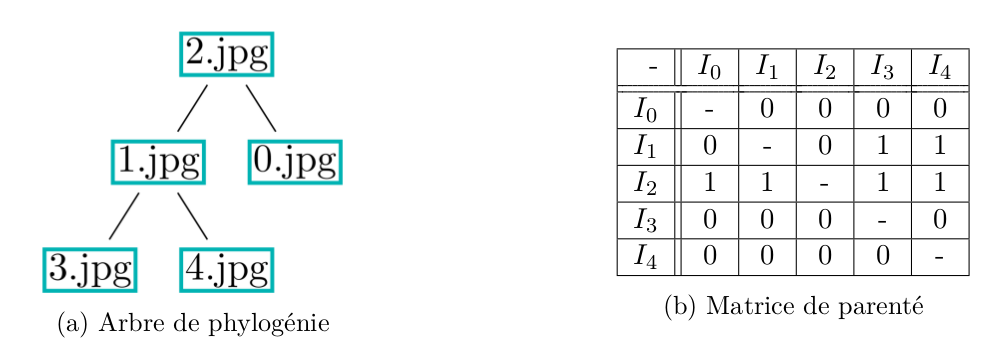
\includegraphics[width=.9\linewidth]{tree_table.png}
  % \centering
%   \subfloat[Arbre de phylogénie\label{Arbre de phylogenie}]{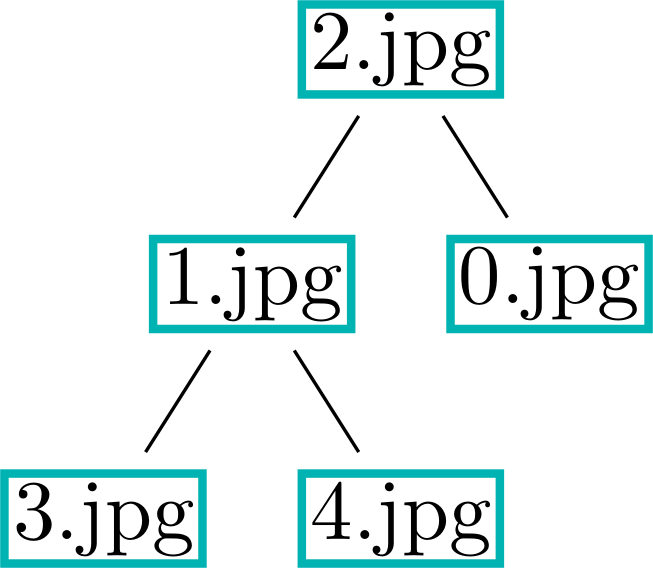
\includegraphics[width=.27\linewidth]{algo_tree.png}}
%   \subfloat[Matrice de parenté\label{fig:b}]{
%     \scalebox{0.75}{
%       \begin{tabular}{|r||c|c|c|c|c|}
%         \hline
%         - & $I_{0}$ & $I_{1}$ & $I_{2}$ & $I_{3}$ & $I_{4}$ \\ \hhline{|=::=|=|=|=|=|}
%         $I_{0}$ & - & 0 & 0 & 0 & 0 \\ \hline
%         $I_{1}$ & 0 & - & 0 & 1 & 1 \\ \hline
%         $I_{2}$ & 1 & 1 & - & 1 & 1 \\ \hline
%         $I_{3}$ & 0 & 0 & 0 & - & 0 \\ \hline
%         $I_{4}$ & 0 & 0 & 0 & 0 & - \\ \hline
%       \end{tabular} 
%     }
% }
%   \caption{A figure}
%   \label{fig:1}
\end{figure}

%   \begin{figure}
%       \centering
%       \subfloat{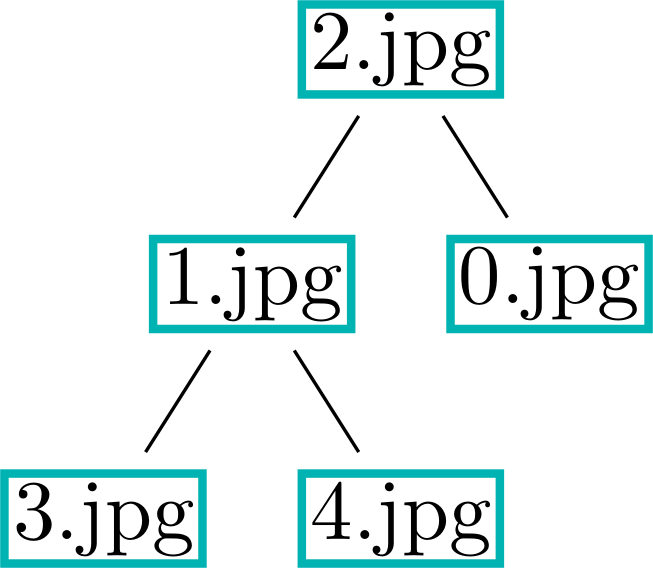
\includegraphics[width=.5\linewidth]{algo_tree.png}}
%       % \caption{Arbre de phylogénie}
%       % \label{algo_tree}
%     % \begin{subfigure}{.5\textwidth}
%       \centering
% \subfloat{
%       \begin{tabular}{|r||c|c|c|c|c|}
%         \hline
%         - & $I_{0}$ & $I_{1}$ & $I_{2}$ & $I_{3}$ & $I_{4}$ \\ \hhline{|=::=|=|=|=|=|}
%         $I_{0}$ & - & 0 & 0 & 0 & 0 \\ \hline
%         $I_{1}$ & 0 & - & 0 & 1 & 1 \\ \hline
%         $I_{2}$ & 1 & 1 & - & 1 & 1 \\ \hline
%         $I_{3}$ & 0 & 0 & 0 & - & 0 \\ \hline
%         $I_{4}$ & 0 & 0 & 0 & 0 & - \\ \hline
%       \end{tabular} 
%       % \caption{Matrice de parenté}
%       % \label{parentage_matrix}
%     % \end{subfigure}
% }
%     \caption{Une arbre de phylogénie et sa matrice de parenté.}
%     \label{parentage_tree}
%   \end{figure}

\end{frame}



\begin{frame}
  \frametitle{Points clés de notre approche}
  \begin{block}{}
    Réduction d'un problème de reconstruction d'un arbre de phylogénie à un problème de \textbf{négation de parenté}
  \end{block}
  \begin{block}{}
    Facilement extensible
  \end{block}
\end{frame}

% \begin{frame}
%   \frametitle{Les marqueurs : facteur de qualité}
%   \centering
%   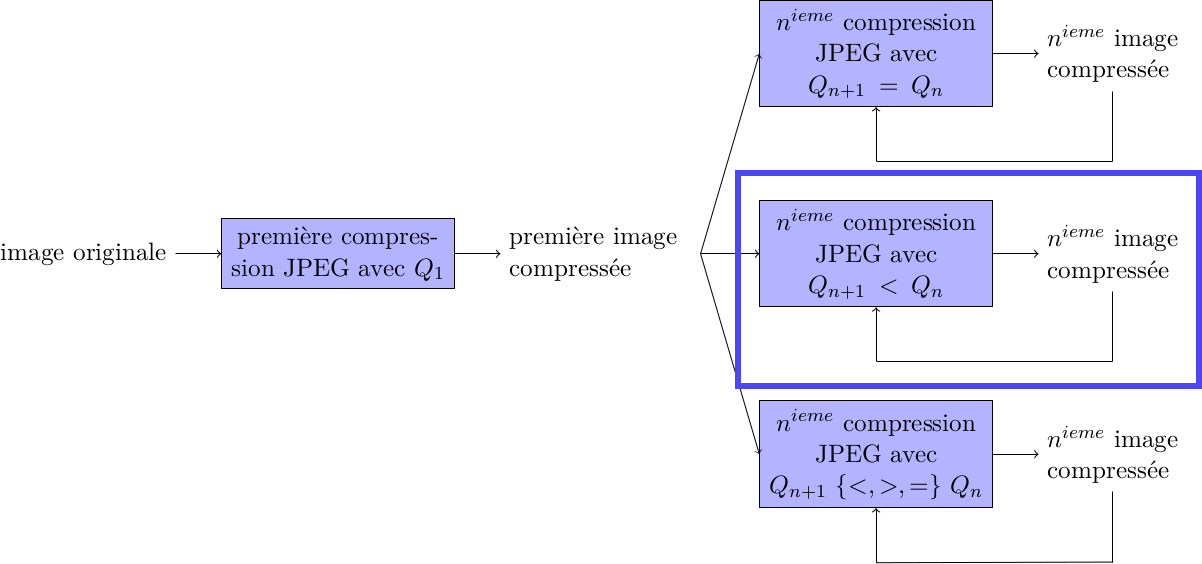
\includegraphics[width=0.8\linewidth]{qinf.png}
%   \begin{block}{}
%     Estimation du facteur de qualité
%   \end{block}
% \end{frame}

% \begin{frame}
%   \frametitle{Les marqueurs : valeurs manquantes dans l'histogramme des coefficients DCT}
%   \begin{block}{}
%     Les coefficients sont des multiples des valeurs de la table de quantification
    
%   \end{block}
%   \begin{figure}
%     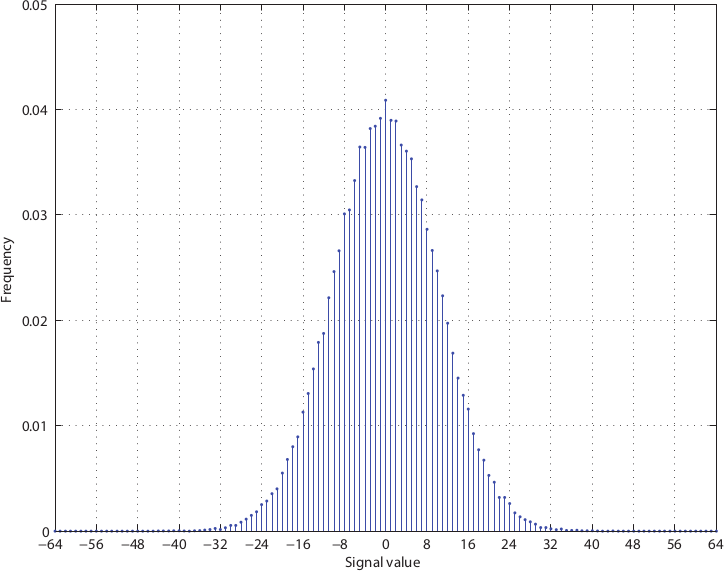
\includegraphics[width=0.5\linewidth]{h1.png}
%     % \caption{Image compressée une fois}
%     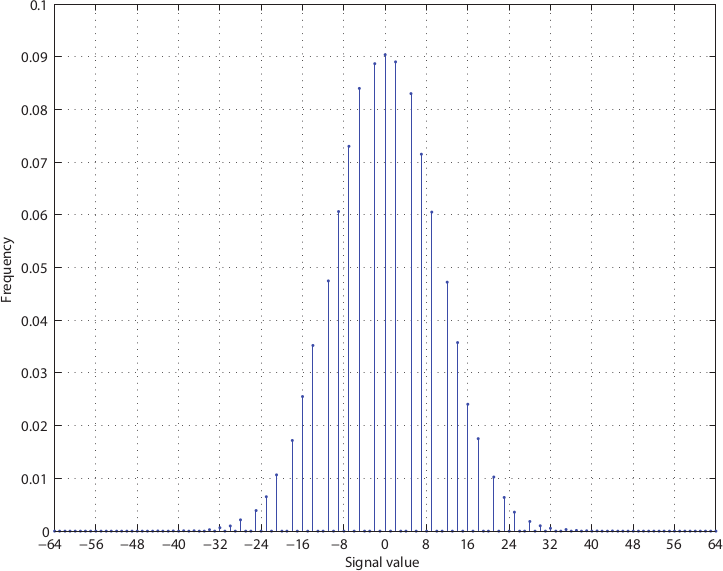
\includegraphics[width=0.5\linewidth]{h2.png}
%     % \caption{\ \ Image simplement compressée - Image doublement compressée, $Q_1 > Q_2$}
%   \end{figure}
% \vspace{-5mm}
% \scalebox{0.7}{
%   \hspace{15mm}
%   \textit{Image simplement compressée}
%   \hspace{18mm}
%   \textit{Image doublement compressée, $Q_1 > Q_2$}
% }  
% \end{frame}

\section{Résultats}
\begin{frame}
  \frametitle{Arbres complets}
  \begin{block}{}
    Une très bonne estimation du $Q_f$
  \end{block}
  \begin{block}{}
    Des métriques proches de 100\%
  \end{block}
  \begin{block}{}
    La précision baisse quand la taille de l'arbre augmente
  \end{block}
\end{frame}

\begin{frame}
  \frametitle{Arbres complets}
  \centering
  \scalebox{0.85}{
  \begin{tabular}{|l||c|c|c|c|c|}
    \hline
     \backslashbox{Métrique}{Dataset}             & \textbf{15 images} & \textbf{25 images} & \textbf{50 images} \\ \hhline{|=::=|=|=|}
    \textbf{\pbox{3.3cm}{Erreur moyenne d'estimation de $Q_f$}} & 0.42 & 0.64 & 0.83 \\ \hhline{|=::=|=|=|}
    \textbf{roots}                                              & 95.83 & 88.88 & 84.72 \\ \hline
    \textbf{edges}                                              & 99.70 & 99.24 & 98.97 \\ \hline
    \textbf{leaves}                                             & 99.59 & 99.15 & 98.74 \\ \hline
    \textbf{ancestry}                                           & 99.44 & 96.88 & 96.96 \\ \hline
  \end{tabular}} 
\end{frame}

\begin{frame}
  \frametitle{Arbres avec une image manquante}
  \begin{block}{}
    Mauvaise estimation de la racine
  \end{block}
  \begin{block}{}
    Bonne estimation du reste de l'arbre
  \end{block}
  \begin{block}{}
    Notre méthode ne détecte que le parent
  \end{block}
\end{frame}

% \begin{frame}
%   \frametitle{Arbres avec une image manquante}
%     \begin{tikzpicture}
%       \node[anchor=south west,inner sep=2] at (0,0) { 
%         \begin{forest}
%           [\href{run:7}{7.jpg}[\href{run:8}{8.jpg}[\href{run:1}{1.jpg}[\href{run:9}{9.jpg}[\href{run:14}{14.jpg}]]][\href{run:13}{13.jpg}[\href{run:3}{3.jpg}[\href{run:5}{5.jpg}]][\href{run:10}{10.jpg}[\href{run:6}{6.jpg}]]]][\href{run:11}{11.jpg}][\href{run:12}{12.jpg}[\href{run:0}{0.jpg}][\href{run:2}{2.jpg}][\href{run:4}{4.jpg}]]]
%         \end{forest}};
%       % \draw[red,ultra thick,rounded corners] (7.5,5.3) rectangle (9.4,6.2);
%       \draw[red, ultra thick](0.8,2.5) -- (2.05,3.1);
%       \draw[red, ultra thick](0.8,3.1) -- (2.05,2.5);
%     \end{tikzpicture}

%     \begin{tikzpicture}
%       \node[anchor=south west,inner sep=2] at (0,0) { 
%         \begin{forest}
%           [\href{run:7}{7.jpg}[\href{run:11}{11.jpg}][\href{run:12}{12.jpg}[\href{run:0}{0.jpg}][\href{run:2}{2.jpg}][\href{run:4}{4.jpg}]]]
%         \end{forest}
%         \begin{forest}
%           [\href{run:1}{1.jpg}[\href{run:9}{9.jpg}[\href{run:14}{14.jpg}]]]
%         \end{forest}
%         \begin{forest}
%           [\href{run:13}{13.jpg}[\href{run:3}{3.jpg}[\href{run:5}{5.jpg}]][\href{run:10}{10.jpg}[\href{run:6}{6.jpg}]]]
%         \end{forest}};
%     \end{tikzpicture}

%     \begin{forest}
%       [\href{run:1}{1.jpg}[\href{run:7}{7.jpg}[\href{run:11}{11.jpg}][\href{run:12}{12.jpg}[\href{run:0}{0.jpg}][\href{run:2}{2.jpg}][\href{run:4}{4.jpg}]]][\href{run:9}{9.jpg}[\href{run:14}{14.jpg}]][\href{run:13}{13.jpg}[\href{run:3}{3.jpg}[\href{run:5}{5.jpg}]][\href{run:10}{10.jpg}[\href{run:6}{6.jpg}]]]]
%     \end{forest}
% \end{frame}

\begin{frame}
  \frametitle{Arbres avec une image manquante}
  % \centering
  \only<1>{
    \begin{tabular}{c|c}
      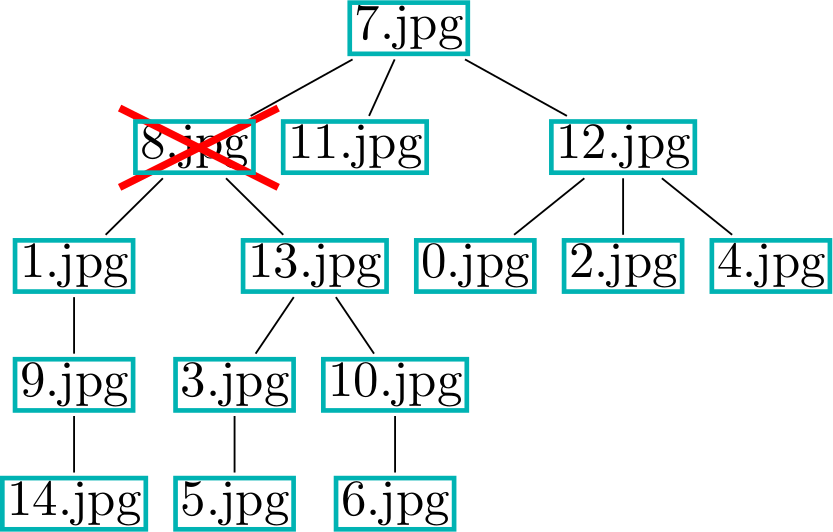
\includegraphics[width=.6\textheight]{tree_cross.png} & 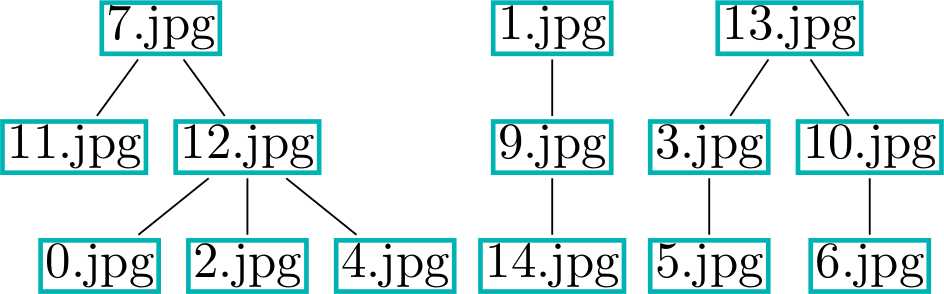
\includegraphics[width=.6\textheight]{3_trees.png} \\
    \end{tabular}
  }
                                                          
  \only<2>{
    \begin{tabular}{c|c}
      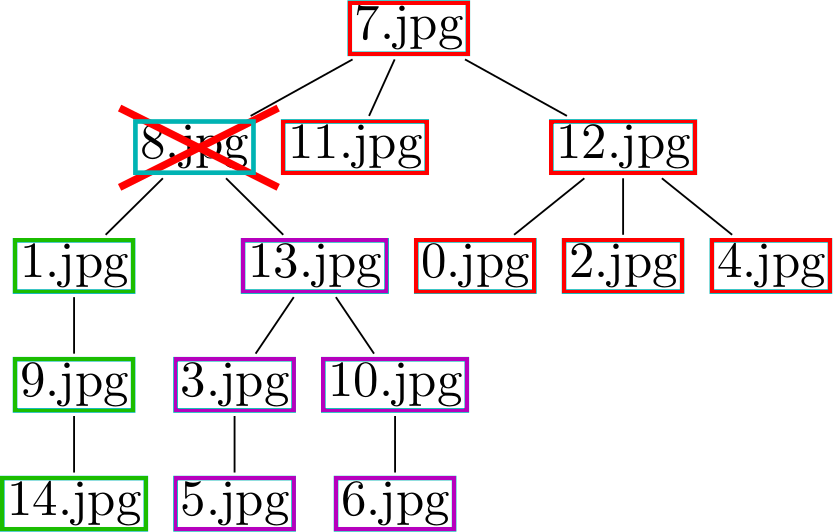
\includegraphics[width=.6\textheight]{tree_cross_color.png} & 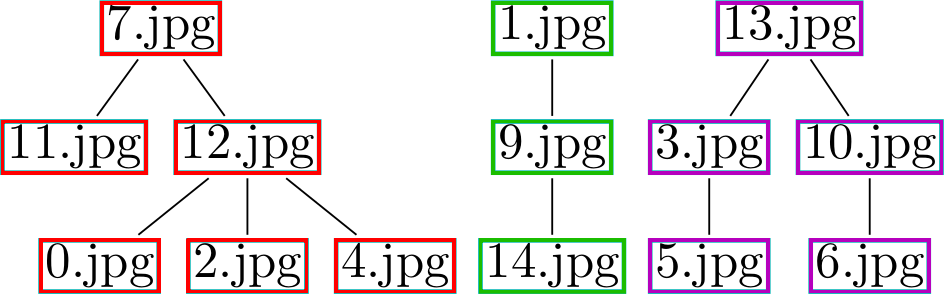
\includegraphics[width=.6\textheight]{3_trees_color.png} \\
    \end{tabular}
  }

\end{frame}

\begin{frame}
  \frametitle{Arbre avec des images en couleur}
  \begin{block}{}
    Aucune adaptation de notre implémentation
  \end{block}
  \begin{block}{}
    Utilisation du canal de luminance
  \end{block}
  \begin{block}{}
    De très bons résultats
  \end{block}
\end{frame}

\begin{frame}
  \frametitle{Arbre avec des images en couleurs}
  \centering
  \scalebox{0.85}{
  \begin{tabular}{|l||c|c|c|c|c|}
    \hline
     \backslashbox{Métrique}{Dataset}             & \textbf{15 images} & \textbf{25 images} & \textbf{50 images} \\ \hhline{|=::=|=|=|}
    \textbf{\pbox{3.3cm}{Erreur moyenne d'estimation de $Q_f$}}         & 1.15  & 1.29  & 1.42  \\ \hhline{|=::=|=|=|}
    \textbf{roots}                                                      & 93.94 & 81.82 & 87.88 \\ \hline
    \textbf{edges}                                                      & 99.35 & 98.61 & 99.38 \\ \hline
    \textbf{leaves}                                                     & 99.62 & 98.66 & 99.78 \\ \hline
    \textbf{ancestry}                                                   & 98.79 & 94.13 & 98.82 \\ \hline
  \end{tabular}}
\end{frame}


  % \begin{block}{}
  %   Détection du parent direct très fiable
  % \end{block}
  % \pause
  % \begin{block}{}
  %   Mauvaise détection des parents éloignés
  % \end{block}
  % \pause
  % \begin{block}{}
  %   Arbre incomplet dans le cas d'images manquantes
  % \end{block}

\section{Conclusion}
\begin{frame}
 \frametitle{Conclusion - perspectives}
 \begin{block}{}
   Une méthode prometteuse
 \end{block}
 \begin{block}{}
   Trouver d'autres marqueurs
 \end{block}
 \begin{block}{}
   Traiter tous les cas de la compression JPEG
 \end{block}
 \begin{block}{}
   Ne pas se limiter à la compression
 \end{block}
\end{frame}

\begin{frame}
  \frametitle{Conclusion - perspectives}
  \centering
\scalebox{3}{
  Des questions ?
}
\end{frame}

\end{document}

